\documentclass[aspectratio=1610]{beamer}

\usepackage[ngerman]{babel}
\usepackage[utf8]{inputenc}
\usepackage[absolute,overlay]{textpos}
\usepackage{hyperref}
\usetheme{lankton-keynote}

\AtBeginSection[]
{
   \begin{frame}
       \frametitle{Outline}
       \tableofcontents[currentsection]
   \end{frame}
}

\title{Das mit der Verschlüsselung}

\author[Mic]{Mic \flq nomaster@chaosdorf.de\frq}

\date[]{25. Januar 2014}

\renewcommand{\quote}[2]
{
  \begin{exampleblock}{}
    {\large “#1”}
    \vskip5mm
    \hspace*\fill{\small--- #2}
  \end{exampleblock}
}


\begin{document}

  \begin{frame}
    \titlepage
  \end{frame}

  \begin{frame}{Zitat}
    \quote{Man is least himself when he talks in his own person.\\
      Give him a mask, and he will tell you the truth.}
      {Oscar Wilde}
  \end{frame}

  \begin{frame}{Privatsphäre}
    Privatsphäre ist…
    \begin{enumerate}
      \pause
      \item Der Bereich der persönlichen Freiheit
      \pause
      \item Das Recht, in Ruhe gelassen zu werden
      \pause
      \item Kontrolle über personenbezogene Daten
      \pause
      \item Verschlüsselung!
    \end{enumerate}
  \end{frame}

  \begin{frame}{Warum kämpfen?}
    “Wer nichts zu verbergen hat, hat auch nichts zu befürchten.”
    \pause
    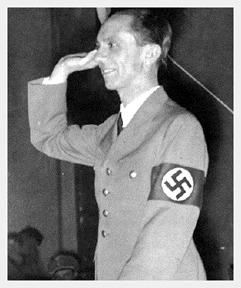
\includegraphics[width=2cm]{goebbels.jpg} 
  \end{frame}

  \begin{frame}{\ldots wie eine Postkarte}
    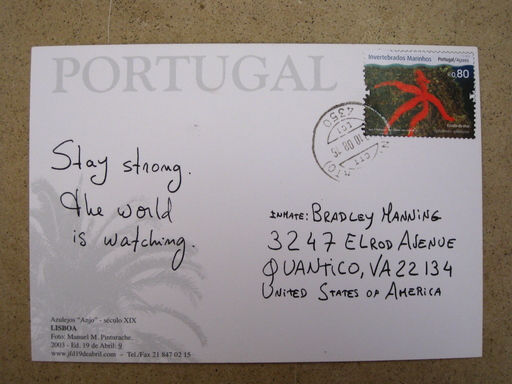
\includegraphics[width=\textwidth]{postcard.jpg}
  \end{frame}

  \begin{frame}{Prinzip Verschlüsselung}
    \begin{columns}
      \begin{column}{.3\textwidth}
        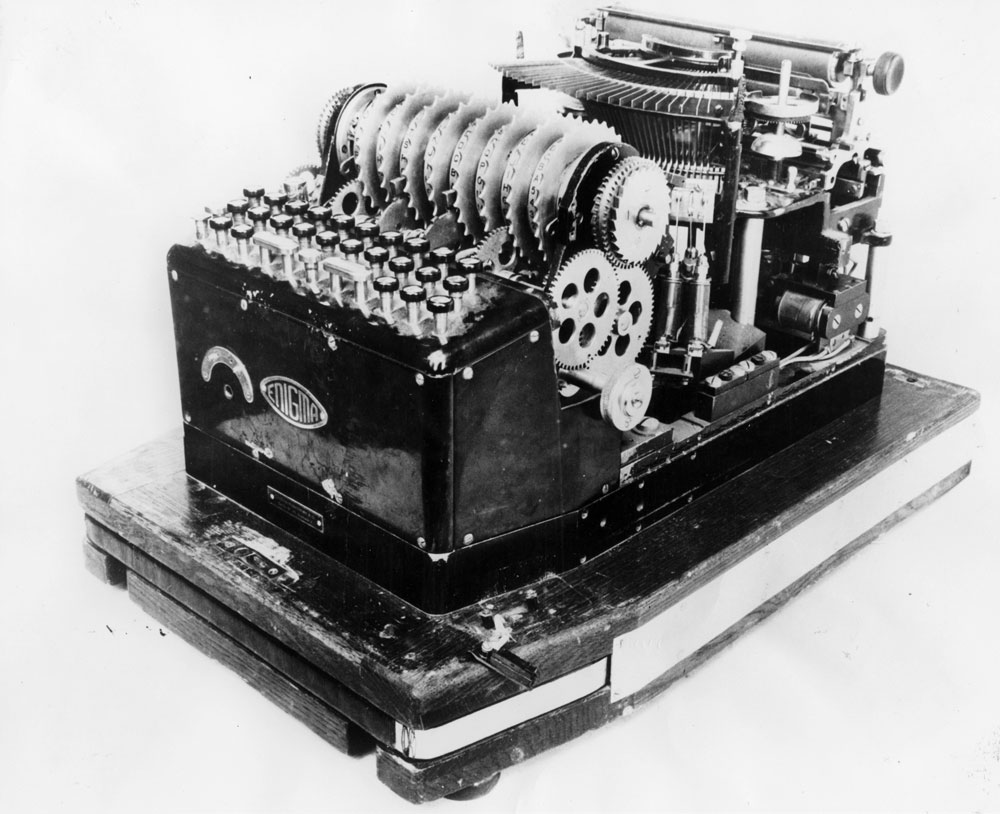
\includegraphics[width=\textwidth]{enigma.jpg}
      \end{column}
      \begin{column}{.7\textwidth}
        \begin{itemize}
          \pause
          \item Kryptographie verbirgt Informationen vor der Öffentlichkeit
          \pause
          \item Ein Geheimnis muss etabliert sein
          \pause
          \item Ohne Vertrauen bringt es nichts
        \end{itemize}
      \end{column}
    \end{columns}
    \pause
    \quote{Traue niemandem!}{anonymous}
  \end{frame}

  \begin{frame}{Sicherheit}
    \quote{Ein System muss auch dann sicher sein,\\wenn das gesamte System
    offen liegt:\\ausgenommen des Geheimnisses.}{Kerckhoff’sches Prinzip}
    \begin{itemize}
      \pause
      \item Die Software muss einsehbar sein.
      \pause
      \item Der Transport kann öffentlich sein.
      \pause
      \item Keine Sicherheit durch Obskurität!
    \end{itemize}
  \end{frame}

  \begin{frame}{Public Key Infrastructure}
    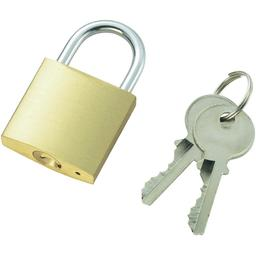
\includegraphics[width=5cm]{key.jpg}
    \pause
    \begin{itemize}
      \item Schlüsselpaar aus öffentlichem und privaten Schlüssel
      \pause
      \item Verschlüsselung mit öffentlichem Schlüssel
      \pause
      \item Signatur mit privatem Schlüssel
    \end{itemize}
  \end{frame}

  \begin{frame}{Erlösung?}
    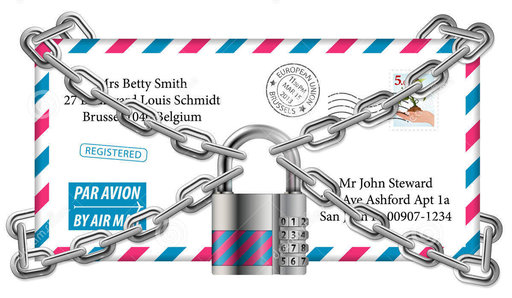
\includegraphics[width=7cm]{mail.jpg}
    \pause
    \begin{itemize}
      \item Verschlüsselung versteckt nur bestimmte Informationen
      \item Metadaten bleiben öffentlich und überwachbar
    \end{itemize}
    \pause
    \quote{Es kommt auf das Angriffsszenario an. Und es ist kompliziert.}{}
  \end{frame}

  \begin{frame}{Schlüsselwerkzeuge}
    \pause
    Verschlüsselung von Datenträgern
    \begin{itemize}
      \pause
      \item TrueCrypt
      \pause
      \item LUKS (Linux)
    \end{itemize}
    \pause
    Verschlüsselung von Nachrichten
    \begin{itemize}
      \pause
      \item OpenPGP mit Enigmail für Thunderbird
      \pause
      \item OpenPGP mit GPGTools für Apple Mail
      \paus
      \item Off-The-Record (OTR) für Pidgin, Adium
    \end{itemize}
    \pause
    Verschlüsselung von Verbindungen
    \begin{itemize}
      \pause
      \item OpenVPN
      \pause
      \item Tor
    \end{itemize}
  \end{frame}

  \begin{frame}{CryptoParty}
    \begin{itemize}
      \item Zeige den Menschen praktische Verschlüsselung
      \pause
      \item Mache es unabhängig und barrierefrei
      \pause
      \item Learning by Doing
      \pause
      \item Have a lot of fun
    \end{itemize}
  \end{frame}
 
 \begin{frame}{Dokumentation}
    Handbücher
    \begin{itemize}
      \pause
      \item CryptoParty Handbook \\ \url{http://www.cryptoparty.in/documentation/handbook}
      \pause
      \item Wikibooks Privacy-Handbuch \\ \url{https://de.wikibooks.org/wiki/Privacy-Handbuch}
    \end{itemize}
  \end{frame}

\end{document}
